\documentclass[ngerman,12pt,parskip=half]{scrreprt}

\usepackage[utf8]{inputenc} %UTF8 Encoding
\usepackage{babel} %Silbentrennung, eingedeutschte 			Verzeichnisnamen, etc
\usepackage[T1]{fontenc} %Lateinisches Alphabet
\usepackage{booktabs} %schöne Tabellen
\usepackage{graphicx} %Bilder
\usepackage{microtype} % Mikrotypografie, mit optischem Randausgleich


\author{Ann-Christin Falkenreck}
\title{Seminararbei Nr.1}

\begin{document}
	\begin{titlepage}
		
	{\large\textbf{Fernuni Hagen \\ Hagen \\ Lehrstuhl für Angewandte Wissenschaften}}
		
	\vspace*{4cm}
		
	{\bfseries\huge Name der Arbeit}
		
	\begin{center}
		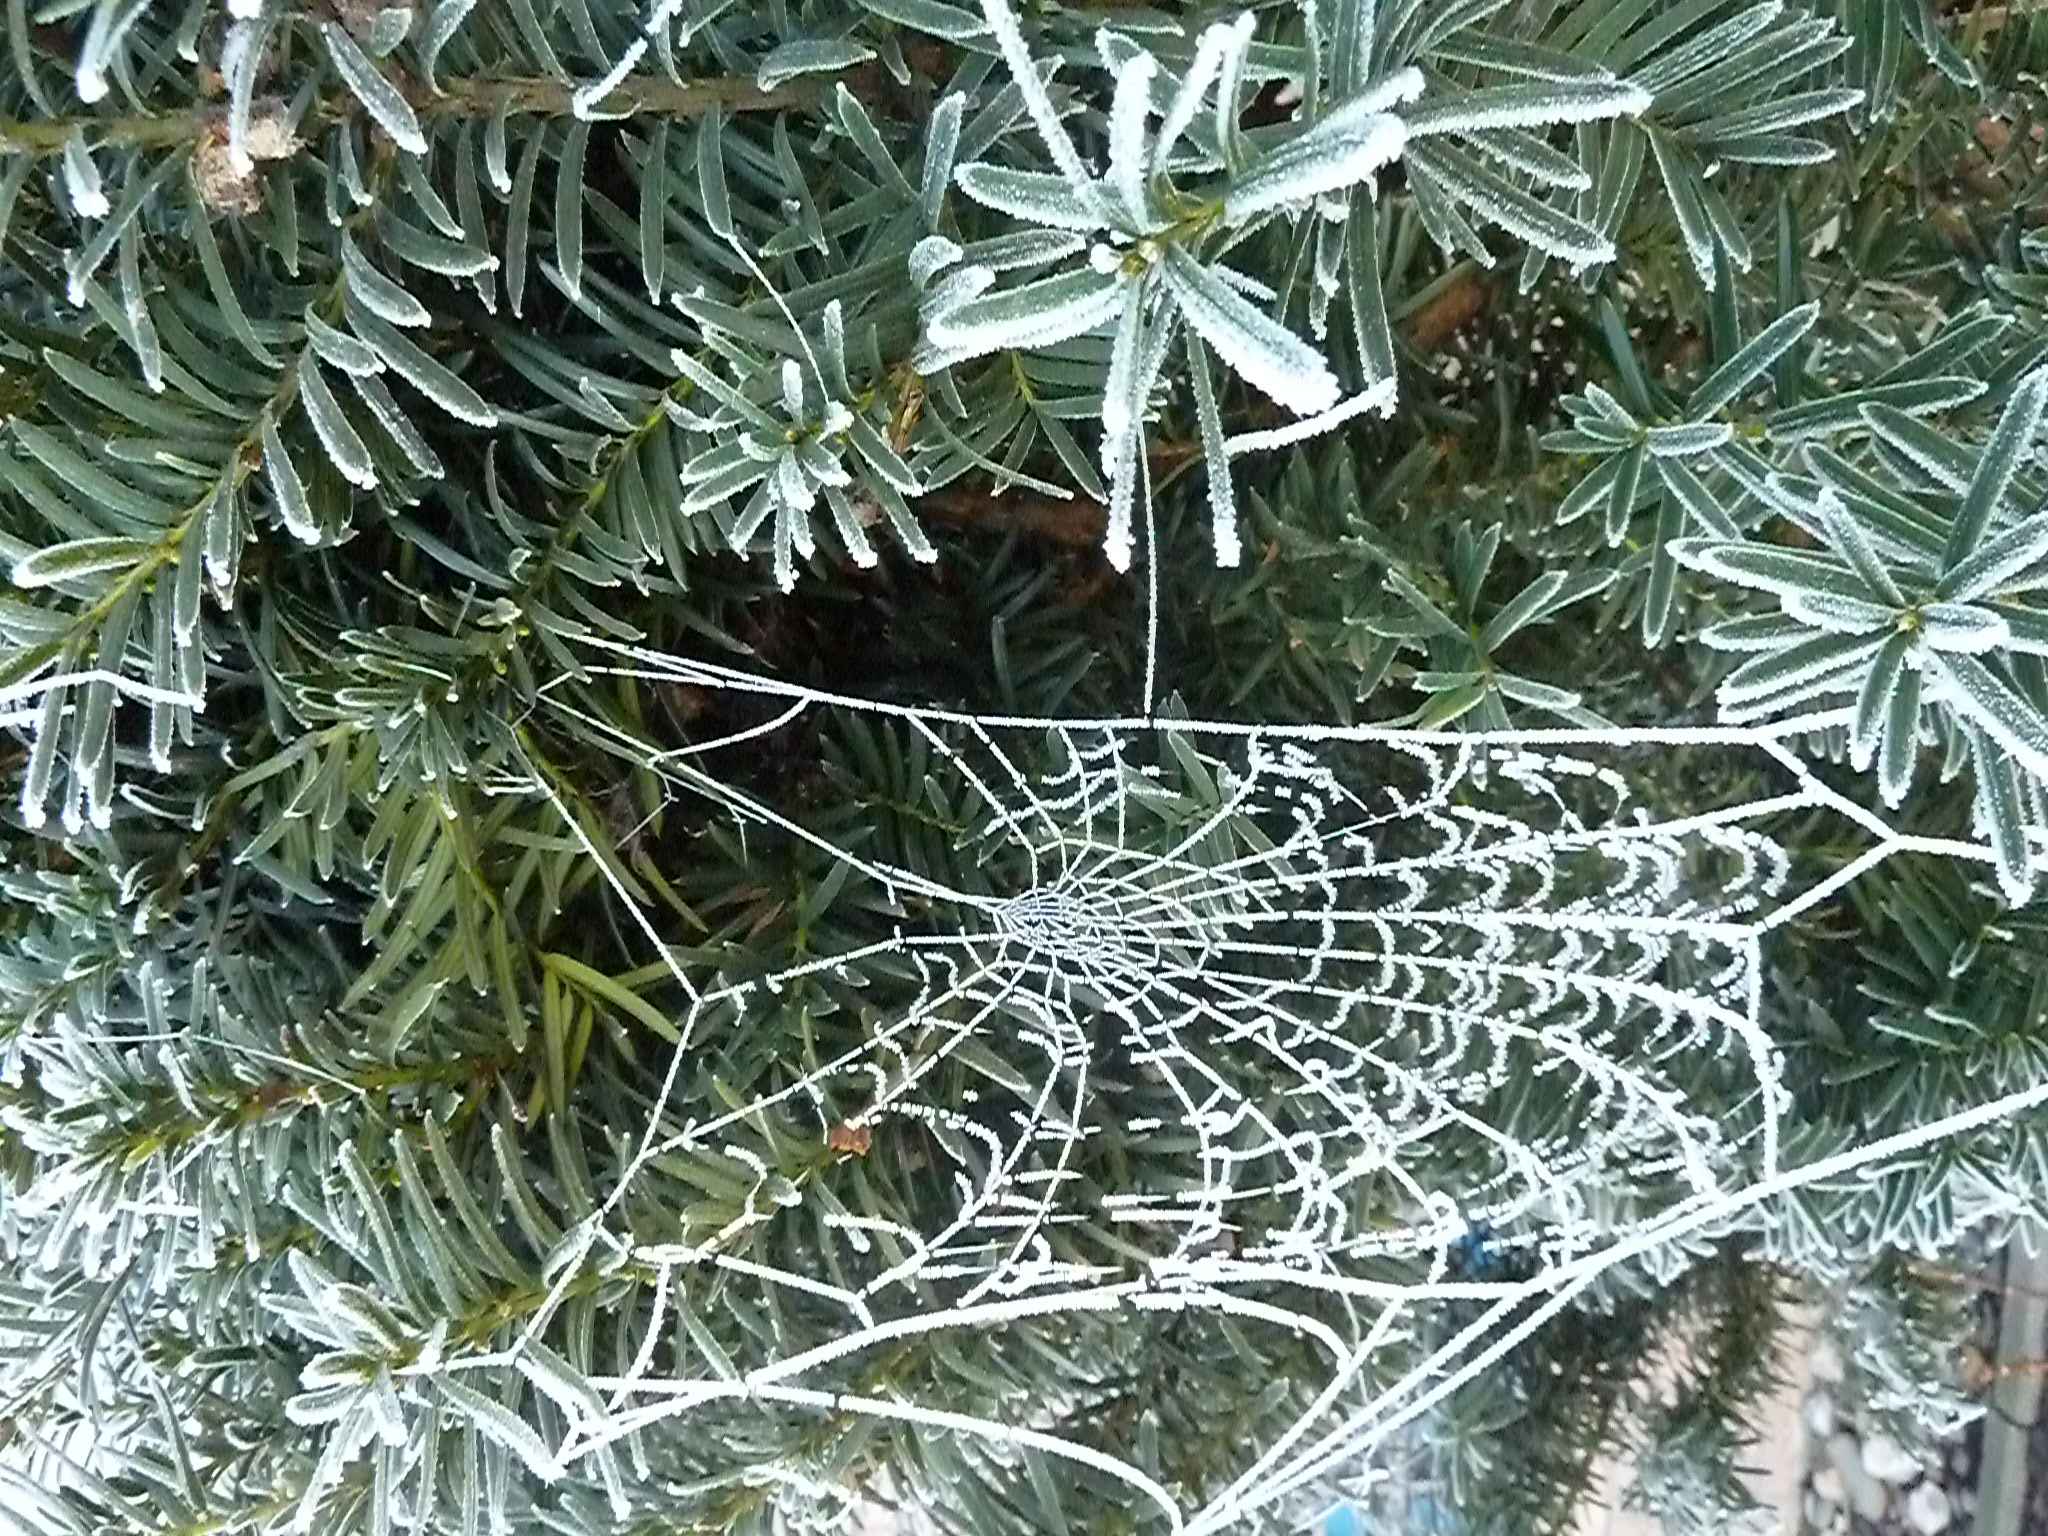
\includegraphics[width=4cm]{Bilder/Herbst}
	\end{center}
		
	\vfill
	Ann-Christin Falkenreck\\
	Matrikelnummer \\
	Lienz, den \today
		
	\end{titlepage}
	
\tableofcontents
\listoffigures
\listoftables
	
\chapter{title}
\section{title}
	\begin{figure}
		\centering
		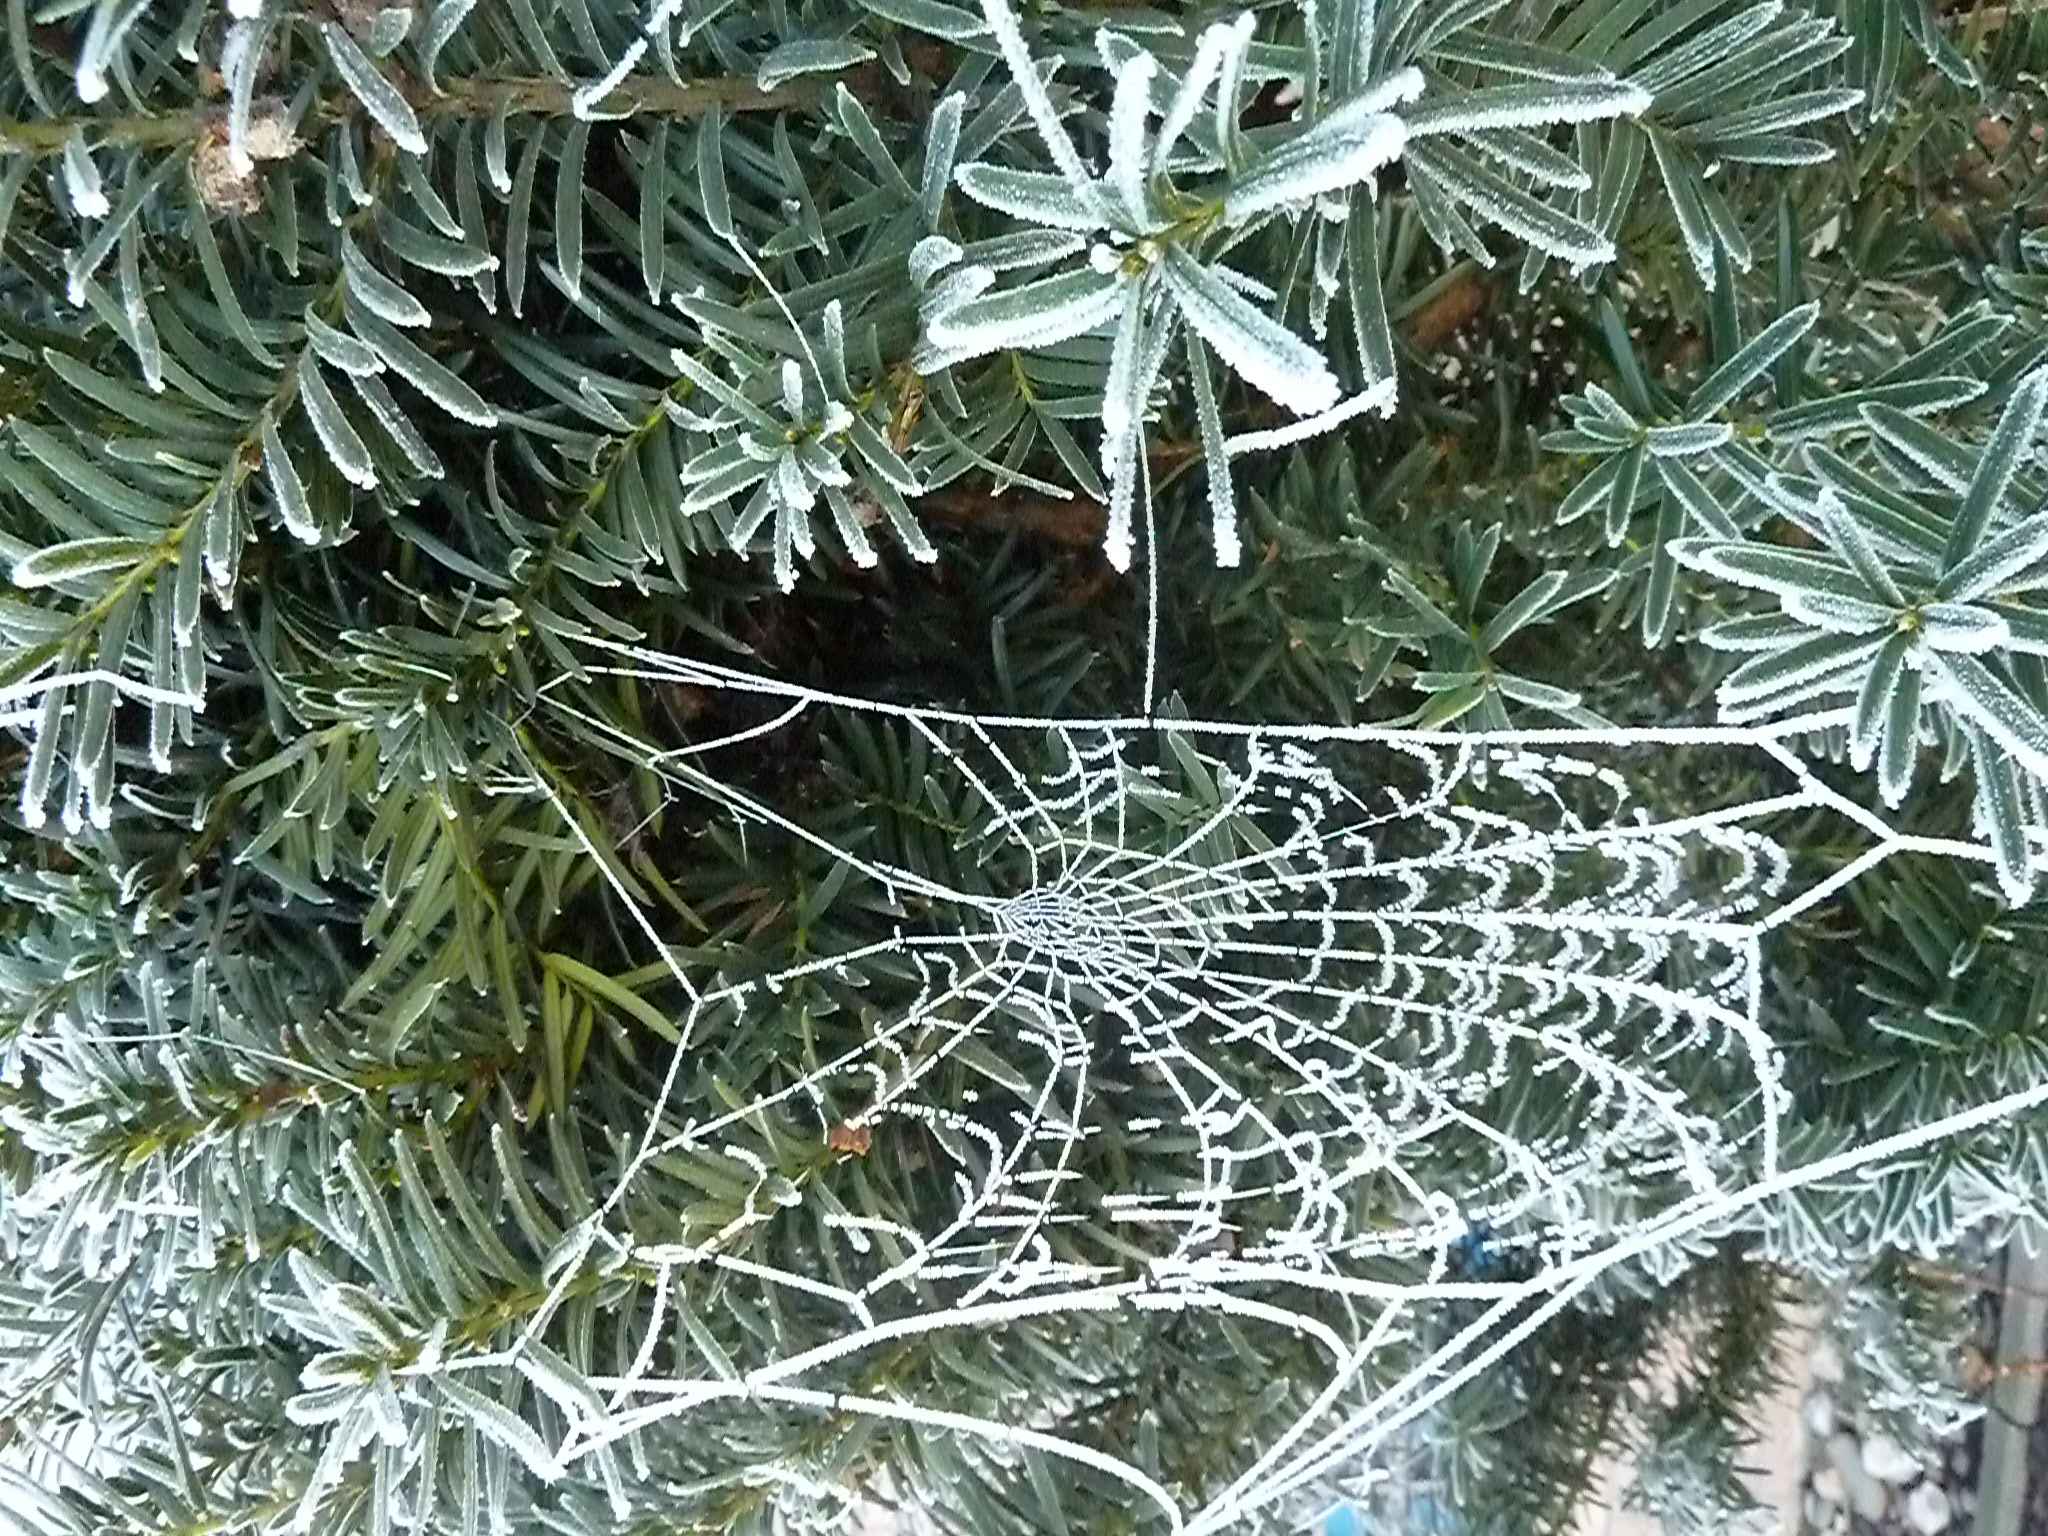
\includegraphics[width=0.75\textwidth]{Bilder/Herbst}
		\caption{Herbst}\label{fig:Herbst}
	\end{figure}

	
	
	
\end{document}